\documentclass[preview]{standalone}
\usepackage{cnn}

\begin{document}
\begin{tikzpicture}[scale=0.4]

	% Input
	\cnnlayer{
		shiftx=0cm,
		dimx=3,%
		dimy=20,%
		dimz=20,%
		label/above=true,
		label/above/text=$3 \times 64 \times 64$,
		label/above/y=2,
		label/below=true,
		label/below/y=2,
		label/below/text=Input,
	}

	% Tail1
	\cnnlayer{
		dimx=3,%
		dimy=20,%
		dimz=20,%
		shiftx=2cm,
		label/above=true,
		label/above/text=$3 \times 64 \times 64$,
		label/above/y=2,
		label/below=true,
		label/below/y=2,
		label/below/text=Conv2D $7 \times 7 / 1$,
	}

	% Tail2
	\cnnlayer{
		dimx=5,%
		dimy=15,%
		dimz=15,%
		shiftx=4cm,
		label/above=true,
		label/above/text=$6 \times 32 \times 32$,
		label/above/y=2,
		label/below=true,
		label/below/y=2,
		label/below/text=MaxPool $3 \times 3 / 2$,
	}

	% Bottleneck A
	\cnnlayer{
		dimx=5,%
		dimy=15,%
		dimz=15,%
		shiftx=7cm,
		label/above=true,
		label/above/text=$6 \times 32 \times 32$,
		label/above/y=2,
		label/below=true,
		label/below/y=2,
		label/below/text=Bottleneck A,
	}

	% Downsample A
	\cnnlayer{
		dimx=7,%
		dimy=12,%
		dimz=12,%
		shiftx=10cm,
		label/above=true,
		label/above/text=$12 \times 32 \times 32$,
		label/above/y=2,
		label/below=true,
		label/below/y=2,
		label/below/text=Downsample A,
	}

	% Bottleneck B
	\cnnlayer{
		dimx=7,%
		dimy=12,%
		dimz=12,%
		shiftx=14cm,
		label/above=true,
		label/above/text=$12 \times 32 \times 32$,
		label/above/y=2,
		label/below=true,
		label/below/y=2,
		label/below/text=Bottleneck B,
	}

	% Downsample B
	\cnnlayer{
		dimx=9,%
		dimy=10,%
		dimz=10,%
		shiftx=19cm,
		label/above=true,
		label/above/text=$24 \times 16 \times 16$,
		label/above/y=2,
		label/below=true,
		label/below/y=2,
		label/below/text=Downsample B,
	}

	% Bottleneck C
	\cnnlayer{
		dimx=9,%
		dimy=10,%
		dimz=10,%
		shiftx=24cm,
		label/above=true,
		label/above/text=$24 \times 16 \times 16$,
		label/above/y=2,
		label/below=true,
		label/below/y=2,
		label/below/text=Bottleneck C,
	}

	% Downsample C
	\cnnlayer{
		dimx=14,%
		dimy=8,%
		dimz=8,%
		shiftx=30cm,
		label/above=true,
		label/above/text=$48 \times 8 \times 8$,
		label/above/y=2,
		label/below=true,
		label/below/y=2,
		label/below/text=Downsample C,
	}

	% Pooling
	\veclayer{
		dimy=8,%
		shiftx=39cm,
		label/above=true,
		label/above/text=$48$,
		label/above/y=2,
		label/below=true,
		label/below/y=2,
		label/below/text=Max/Avg Pool,
	}

	% Head
	\veclayer{
		dimy=8,%
		shiftx=41cm,
		label/above=true,
		label/above/text=$10$,
		label/above/y=2,
		label/below=true,
		label/below/y=2,
		label/below/text=Fully Connected + Softmax,
	}
\end{tikzpicture}
\end{document}
